Parte del análisis, en concreto los patrones de de diseño, se investigó en paralelo que la implementación, cuando algo resultaba no ser como creíamos había que revisar lo comprendido de analizar el código de la aplicación. Por ello esta sección pretende parte el marco teórico del proyecto aprendido de observar el código de Bitwarden. Mientras que más adelante se discutirá la parte práctica. Por tanto el orden aquí expuesto no representa el orden cronológico del proyecto.

\subsubsection{Historias de usuario}
\begin{itemize}
    \item Cernuda es un joven al que le encanta ver a sus creadores de contenido favoritos, como Ibai, AuronPlay o ElRubius. Para verlos usa la plataforma \textit{Twitch}. Cernuda quiere iniciar sesión en su \textit{Smart TV}, pero como usuario de Bitwarden su clave es muy larga y por lo tanto tosca de introducir con el mando a distancia.
    \item Lorca es un fanático de los videojuegos, recientemente se ha comprado la nueva consola de última generación PlayStation 5. Lorca quiere iniciar sesión en PlayStation Network, pero como usuario de Bitwarden conoce poco más que su clave maestra. Al igual que Cernuda, su clave de un servicio web es demasiado larga y resulta molesto introducirla en el dispositivo.
    \item Góngora es un estudiante de informática. Entre el estudio para las asignaturas y cursos de la universidad, suele usar ordenadores de la biblioteca y el "Gaming Space ULPGC". Por ello tiene que iniciar sesión con frecuencia en GitHub y otros sitios webs, sin embargo esto requiere muchos pasos, iniciar sesión en Bitwarden, copiar la clave al portapapeles y luego pegarla en el campo para iniciar sesión. Además teme que previamente alguien haya activado el historial del portapapeles de Windows y un día se olvide de comprobarlo.
    \item Quevedo es un trabajador que frecuenta múltiples oficinas, por lo tanto requiere iniciar sesión con frecuencia en ordenares distintos, al igual que Góngora le resulta que son demasiados pasos los necesarios hasta poder iniciar sesión.
\end{itemize}

Adicionalmente están estas solicitudes por parte de usuarios de Bitwarden de realizar lo que se plantea en este proyecto:
\begin{itemize}
    \item \url{https://community.bitwarden.com/t/does-bitwarden-android-support-logging-in-via-bluetooth/9364/3}
    \item \url{https://community.bitwarden.com/t/add-inputstick-api-to-apps-ios-android/3041}
    \item \url{https://community.bitwarden.com/t/inputstick-integration/42596}
\end{itemize}

\subsubsection{Modificaciones en la GUI}

Para desarrollar una solución es primero necesario hacer un análisis. Como el objetivo es hacer parecer que la funcionalidad siempre estuvo en la aplicación, lo primero será buscar en qué contexto puede ser necesario escribir una clave desde la aplicación mediante InputStick. Empezaremos por lo más trivial, el usuario ya tiene una \gls{cuenta} creada y quiere escribir la clave de forma inalámbrica, para ello, el usuario navegará hasta el \gls{login} \cite{item}, donde se encuentra la pantalla de la Figura \ref{fig:bitapp-login-view}.

\begin{figure}[H]
    \centering
    \frame{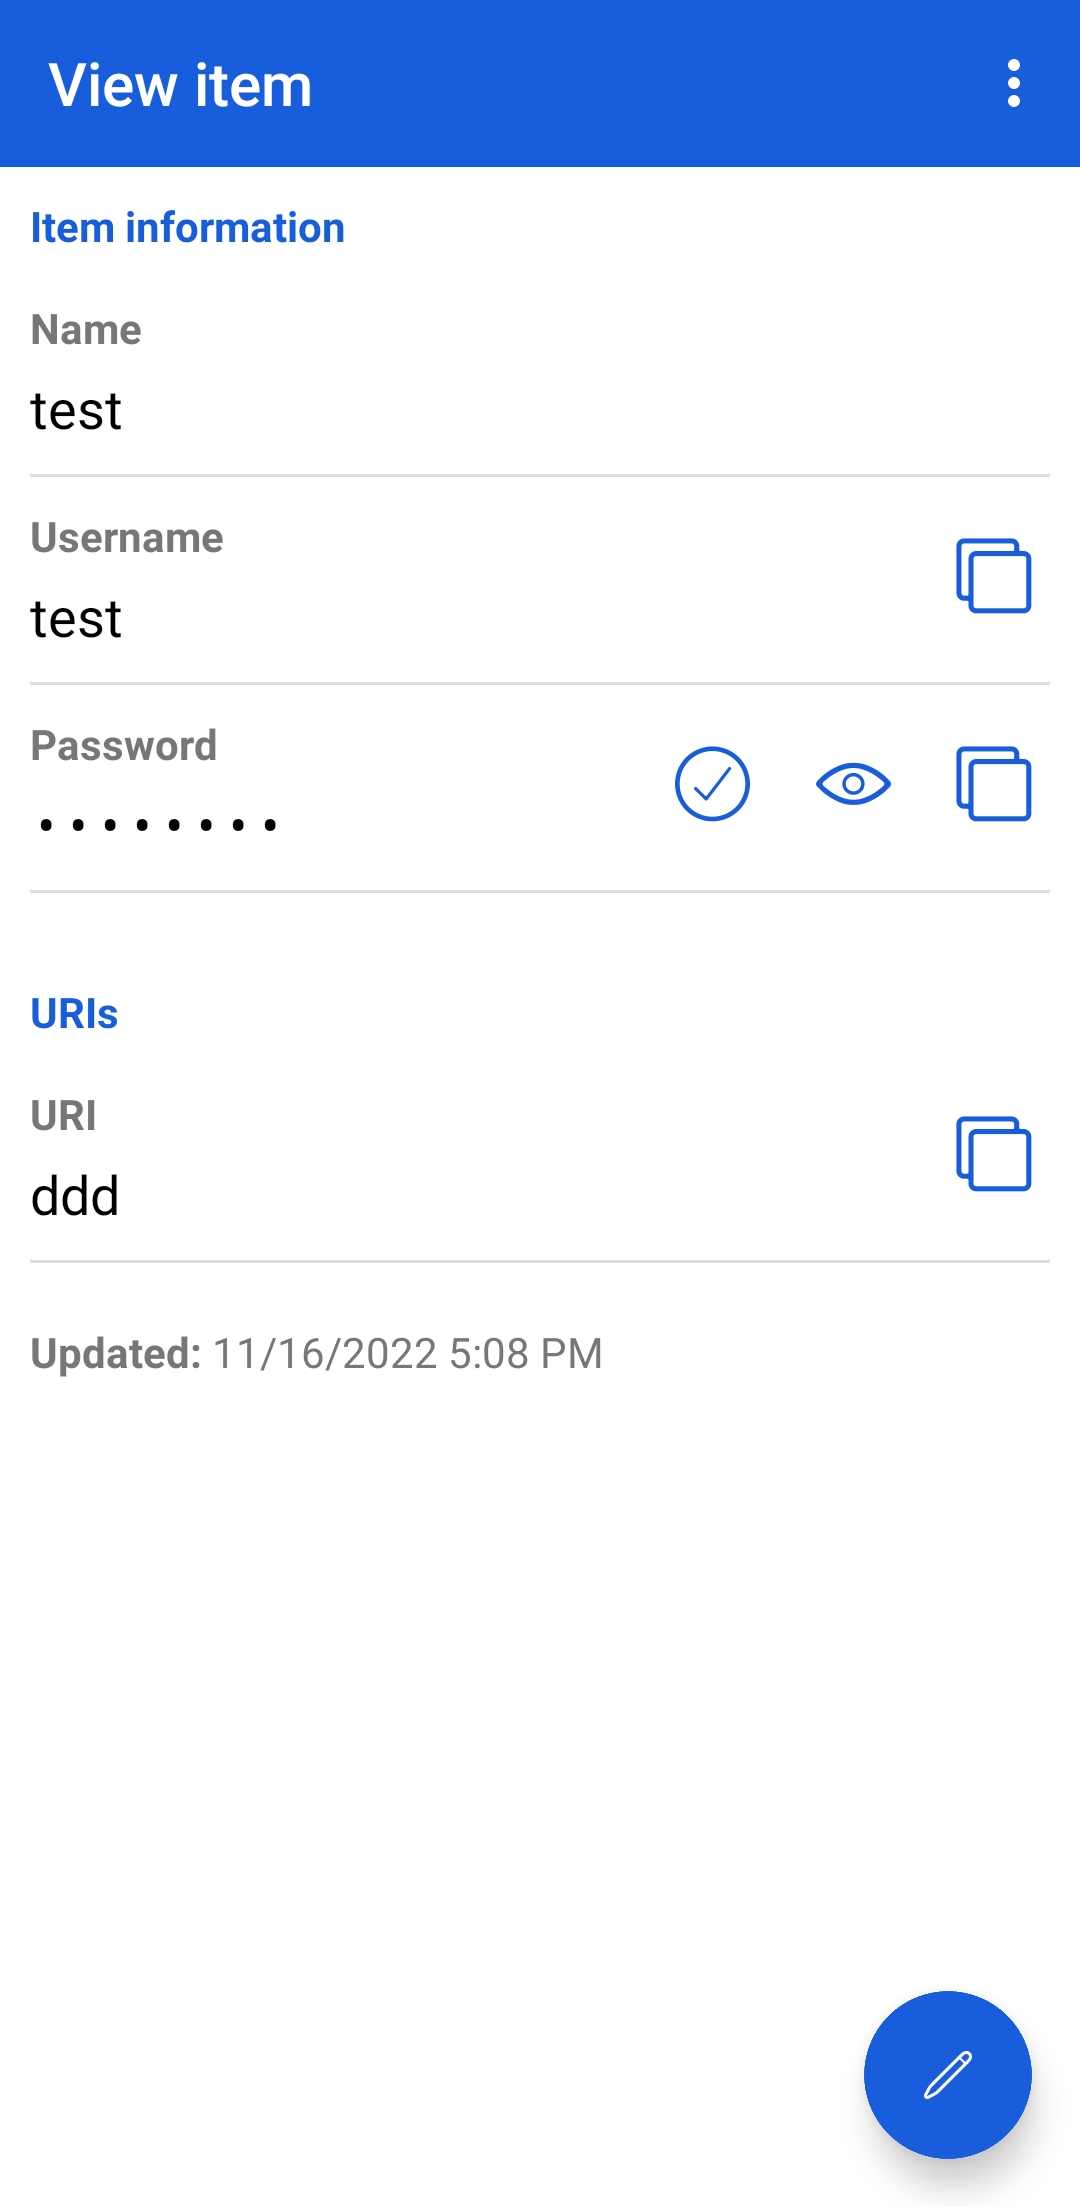
\includegraphics[width=0.4\columnwidth]{gfx/bitapp/bitapp-login-view.png}}
    \caption{pantalla de un \gls{login}. \href{https://play.google.com/store/apps/details?id=com.x8bit.bitwarden}{De la app de Bitwarden.}}
    \label{fig:bitapp-login-view}
\end{figure}

Podemos observar que el campo \textit{Password}, tiene diferentes botones, en orden de izquierda a derecha:
\begin{itemize}
    \item Comprobar clave:
    Comprueba si la clave ha sido comprometida mediante la \gls{api} de \textit{Have I Been Pwned}. \cite{pwnedpasswords}% descubierto analizando las queries con tracker control
    \item Alternar visibilidad:
    Alterna el enmascaramiento de la clave.
    \item Copiar clave:
    Copia la clave al portapapeles.
\end{itemize}
De aquí podemos extraer que cada vez que haya un botón para copiar al portapapeles es un caso de uso donde el usuario podría querer escribir de forma inalámbrica su clave. Como en la imagen no sólo hay un botón para copiar al portapapeles la clave, sino que lo hay también para el usuario y el \gls{uri} podemos entender que sería útil escribir inalámbricamente también estos campos. Por lo que ahora en el proyecto para lograr uno de los objetivos deberemos tener en cuenta dichas situaciones. Pasaremos pues a buscar en todas las pantallas de la aplicación, cuáles tienen botones para copiar al portapapeles. Esto además mejora la comodidad del producto, pues ni siquiera nos habíamos planteado la opción de enviar el \gls{uri}, lo cual si bien no ahorra mucho tiempo, el poco que ahorra hace que la interacción sea fluida, lo cual, consideramos extremadamente importante.

\begin{figure}[H]
    \centering
    \subfigure[]{\frame{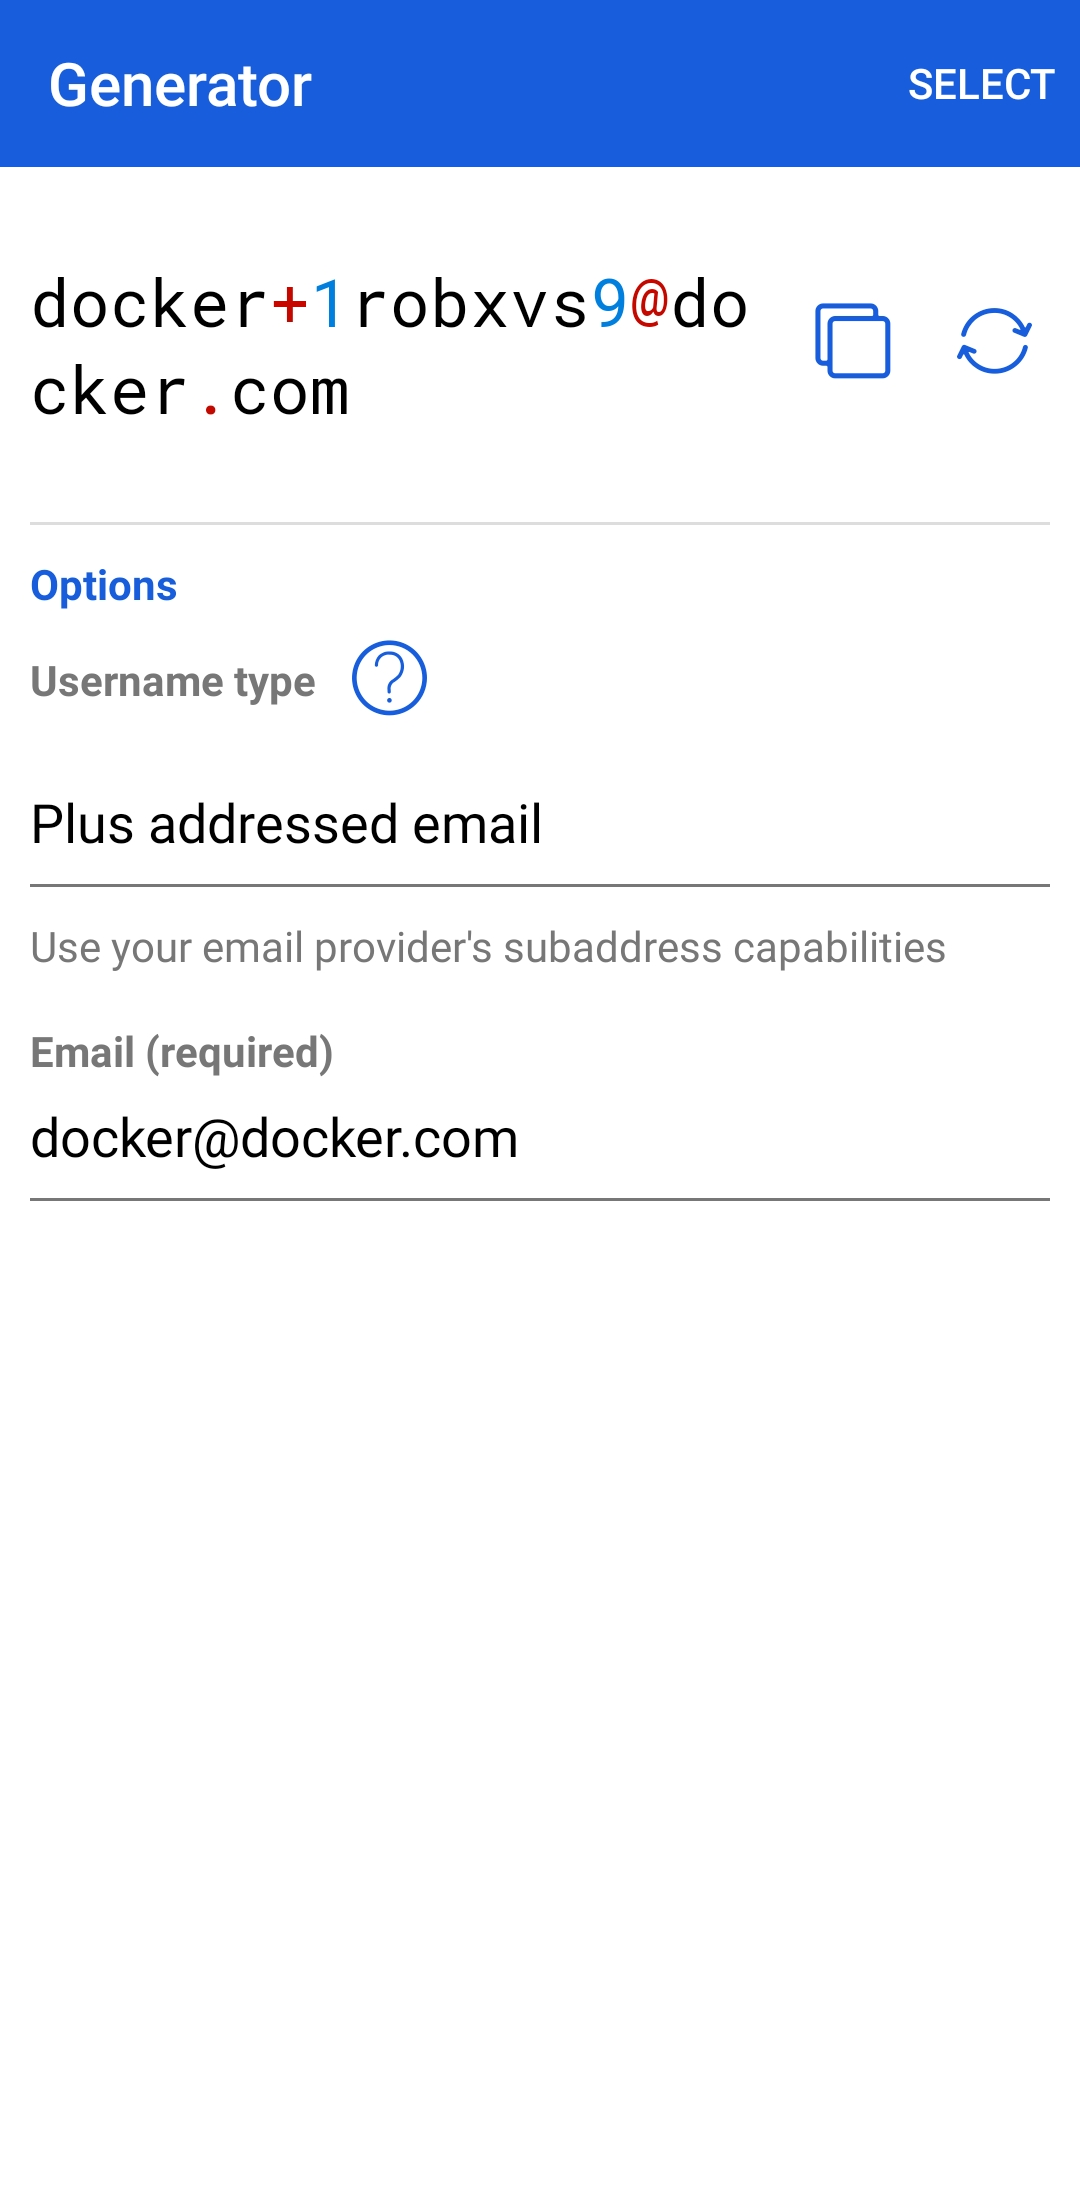
\includegraphics[width=0.24\columnwidth]{gfx/bitapp/bitapp-alias-generator-forced}}}
    \subfigure[]{\frame{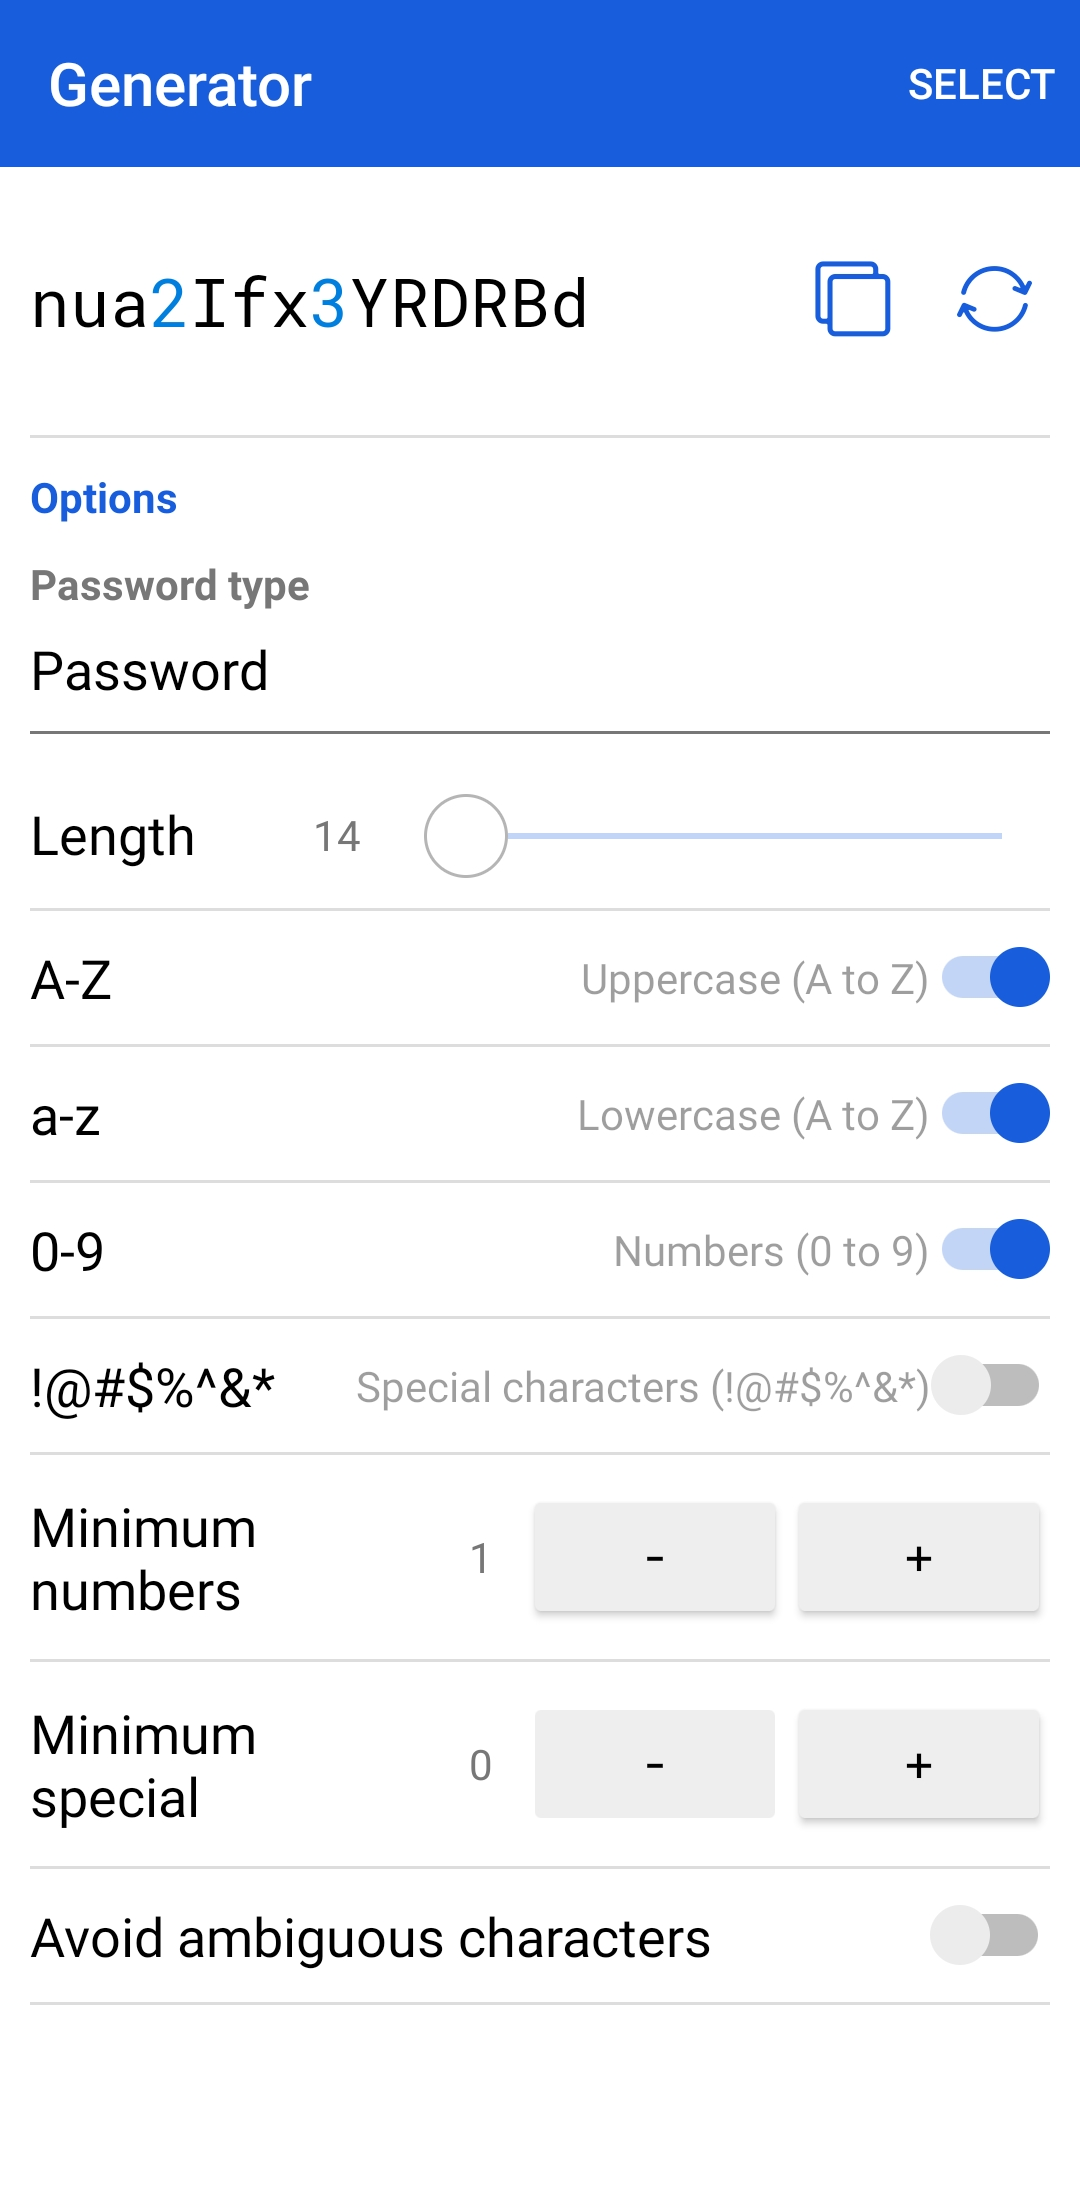
\includegraphics[width=0.24\columnwidth]{gfx/bitapp/bitapp-password-generator-forced}}}
    \subfigure[]{\frame{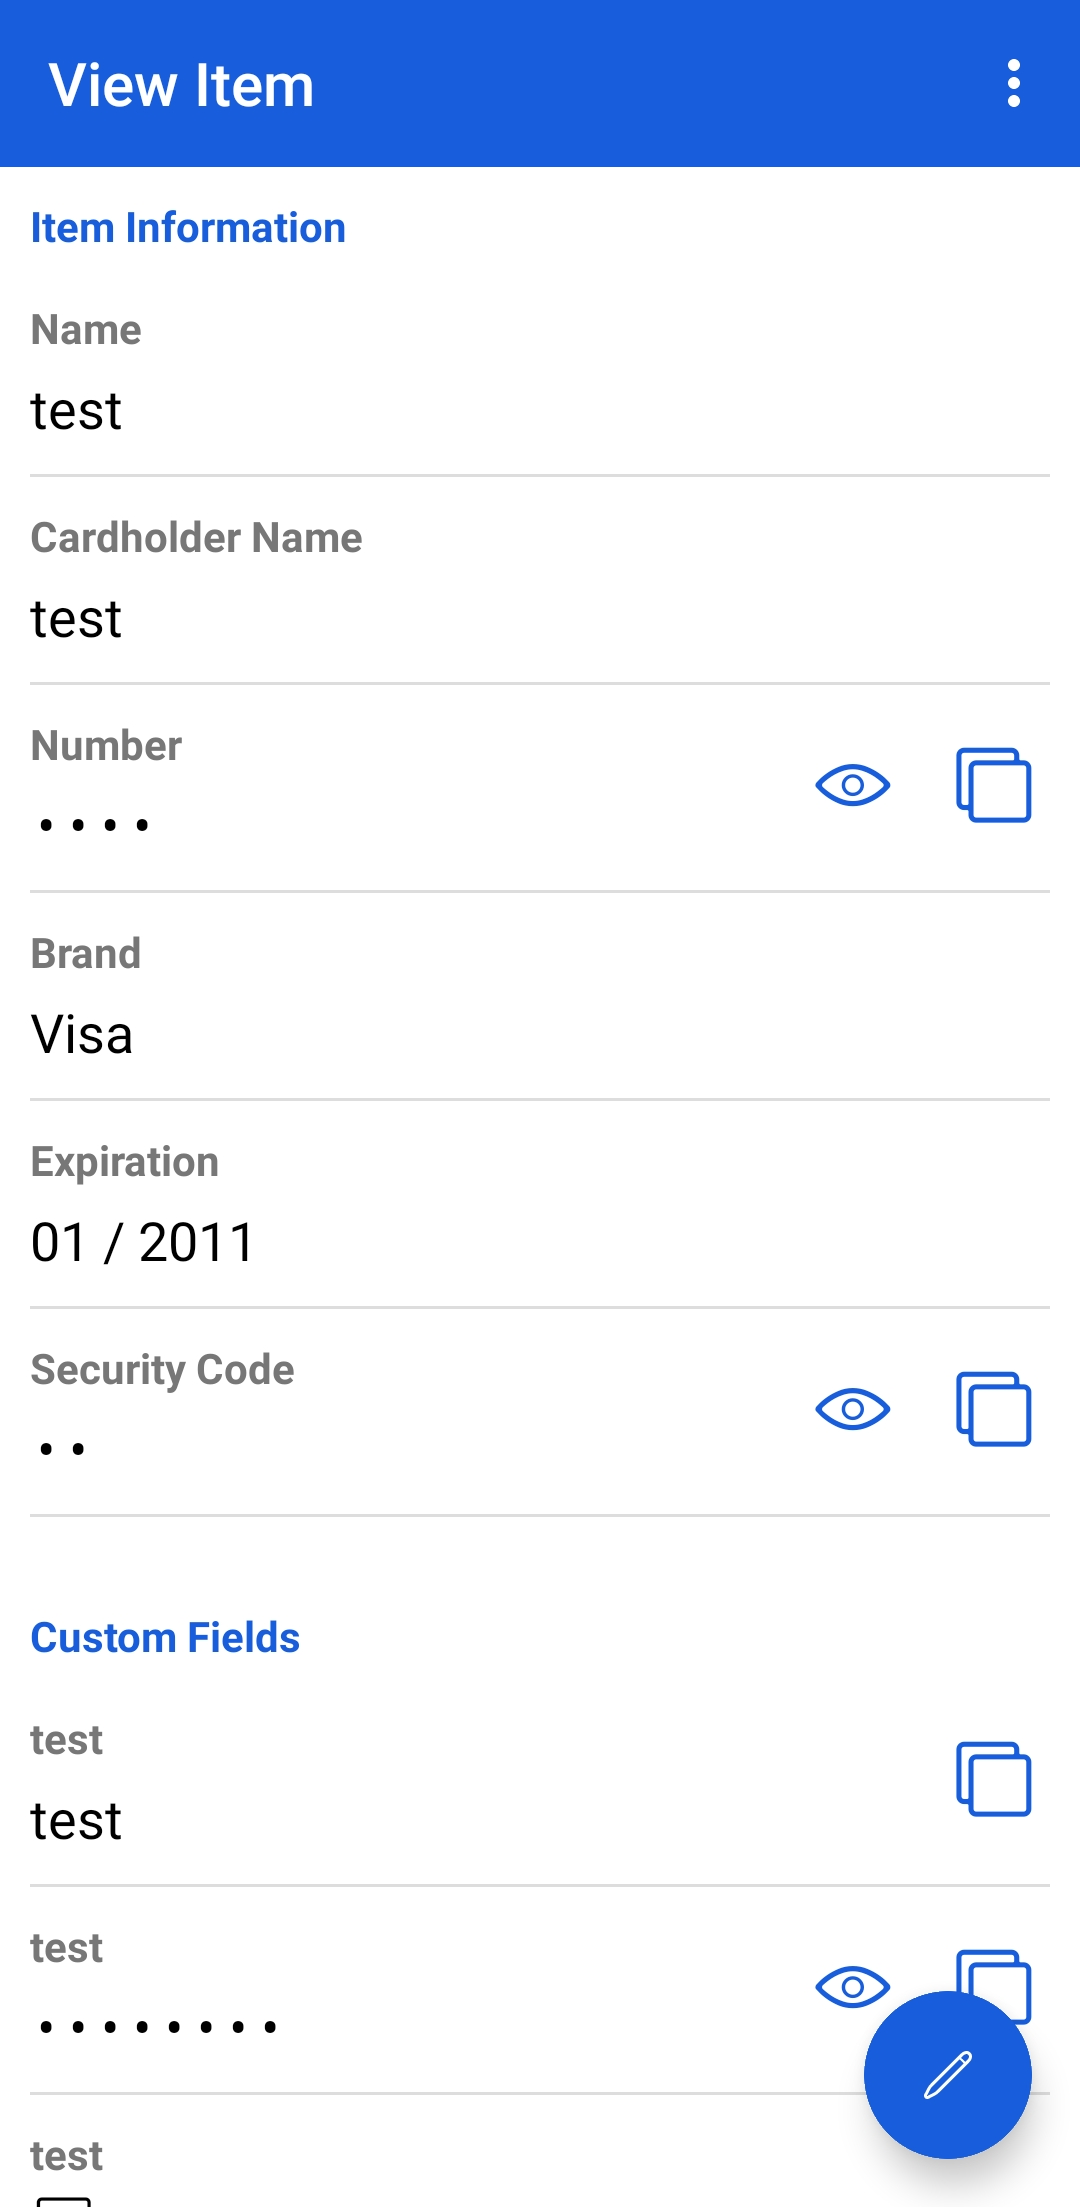
\includegraphics[width=0.24\columnwidth]{gfx/bitapp/bitapp-custom-fields-card-view}}}
    \subfigure[]{\frame{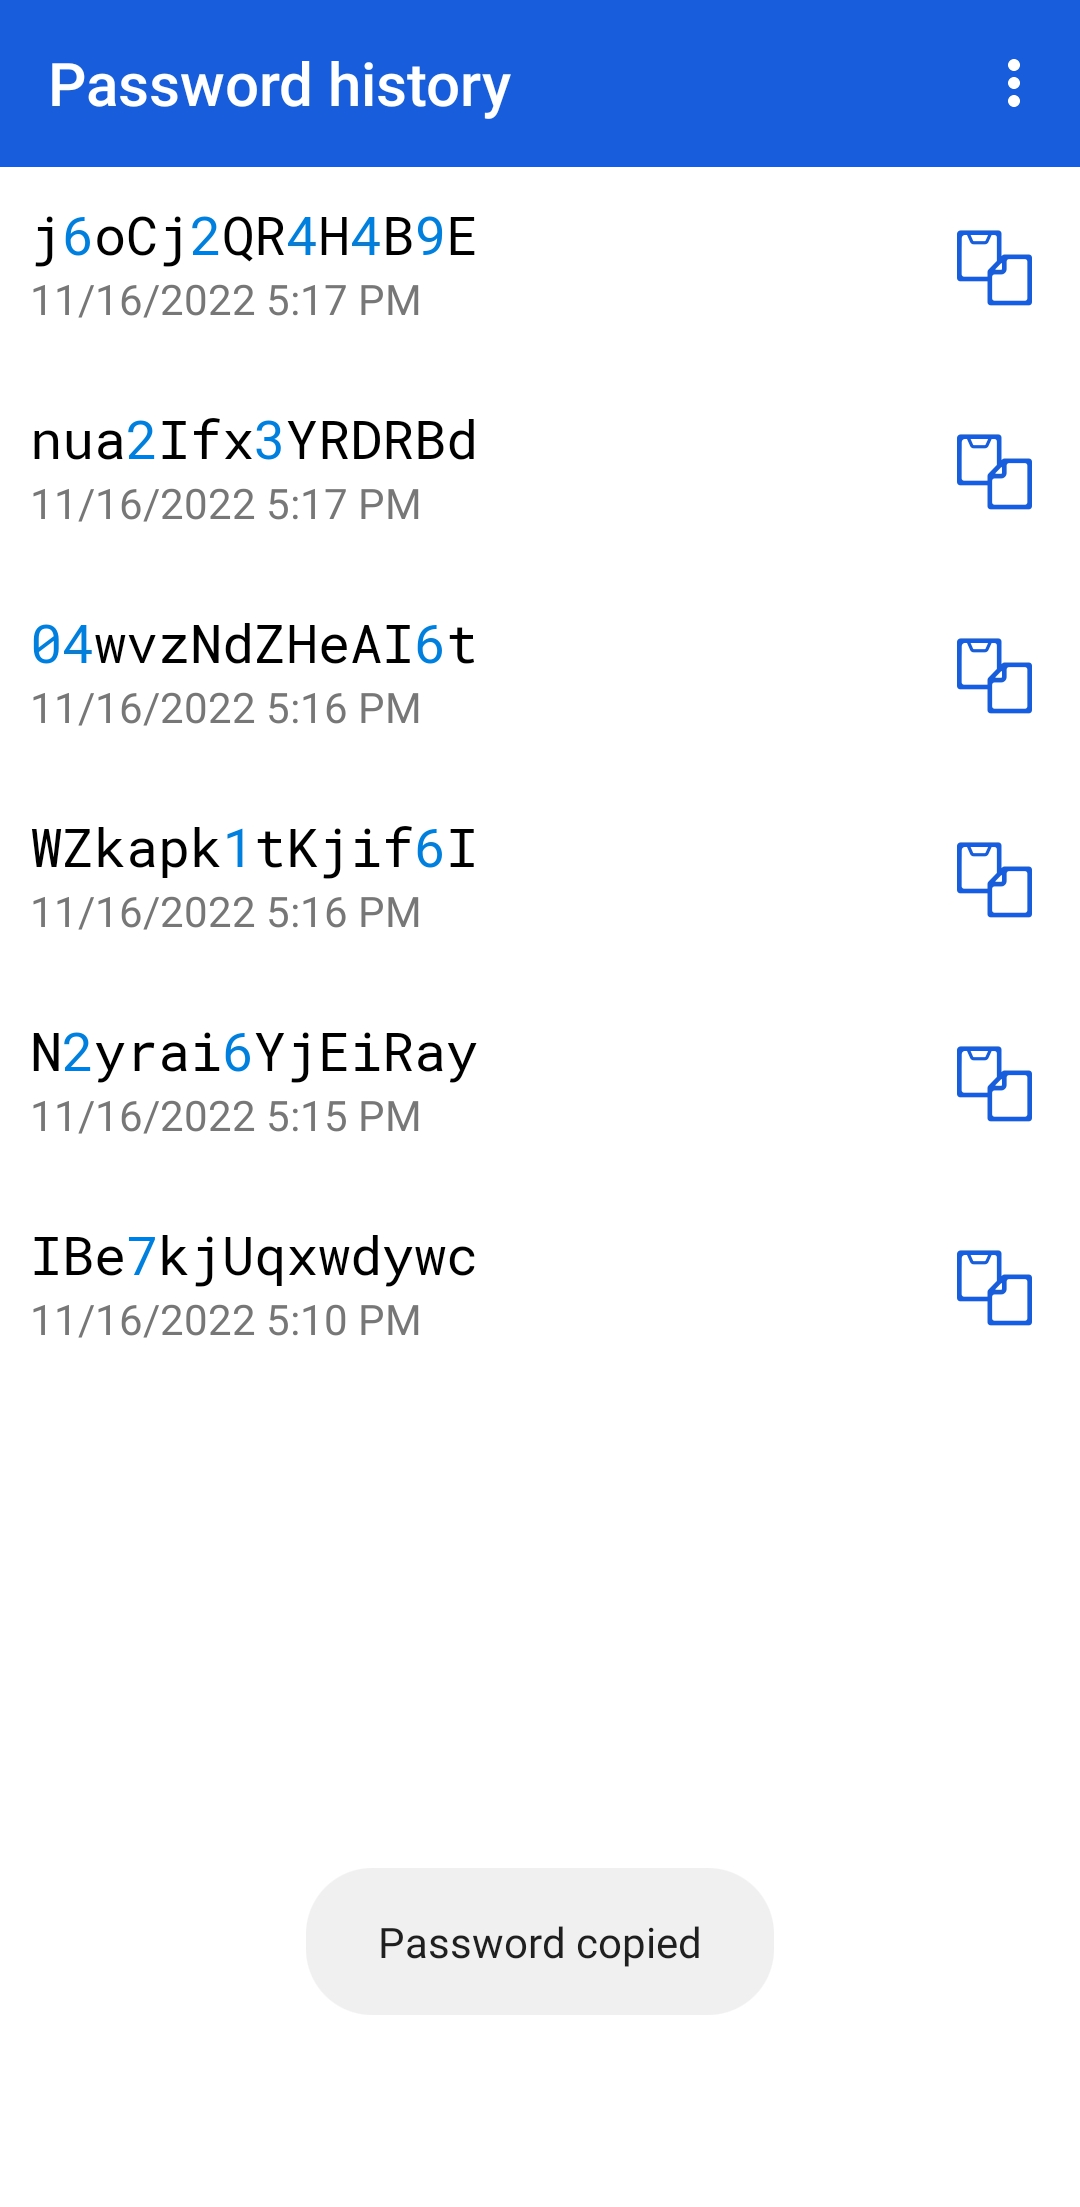
\includegraphics[width=0.24\columnwidth]{gfx/bitapp/bitapp-password-history}}}
    \caption{
        Figura múltiple. \href{https://play.google.com/store/apps/details?id=com.x8bit.bitwarden}{De la app de Bitwarden.} \newline
        \tab (a) pantalla de generación de alias. \newline
        \tab (b) pantalla de generación de claves. \newline
        \tab (c) pantalla de tarjetas, con campos adicionales. \newline
        \tab (d) pantalla de historial de claves.
        }
    \label{fig:bitapp-copy}
\end{figure}
%bitapp-custom-fields-login-view
%bitapp-generator-1-pass
%bitapp-generator-2-alias
%bitapp-password-generator-forced
%bitapp-alias-generator-forced
%bitapp-password-history

Como podemos ver en la Figura \ref{fig:bitapp-copy}, este botón lo podemos encontrar en las pantallas de generación de claves o alias, la vista de tarjeta y el historial de claves, además de la ya mencionada vista de \gls{login}. Así que estas serán las partes que modificaremos para ello.

Lo siguiente es buscar dónde añadir la configuración de InputStick, ya que es necesario poder elegir la velocidad de escritura, así como la disposición, pues el protocolo \gls{hid} no transmite caracteres, si no un código que se corresponde con la ubicación física de la tecla que se ha pulsado, el estándar usa como base una disposición de Estados Unidos, y cualquier otra disposición es en realidad o bien un mapa posición$\longleftrightarrow$carácter creado por el Sistema Operativo o bien un mapa carácter$\longleftrightarrow$posición creado por el dispositivo de entrada\cite{microsofthid}\cite{usbhid}. Como un dispositivo \gls{hid} no puede conocer este mapa, y el Sistema Operativo tampoco, el estándar es que el Sistema Operativo interpreta esta información, un teclado comunicará los códigos de las teclas, y el usuario debe ajustar en el Sistema Operativo cuál debiese ser esta, por lo general esto se hace automáticamente al configurar el idioma\cite{microsoftchangelayout}. Por ello es crucial implementar una forma de cambiar este ajuste, ya que si no se hace, habría que cambiar en el Sistema Operativo la disposición cada vez que se quiera introducir una clave con InputStick y muchas contraseñas se escribirían incorrectamente si no se cambia, pues aunque gran parte del abecedario y los números coinciden entre diferentes disposiciones, el resto de caracteres no suelen coincidir. Lo podemos ver en el siguiente ejemplo interactivo:
\begin{itemize}
    \item \hyperlink{https://learn.microsoft.com/en-us/globalization/keyboards/kbdsp}{Disposición de España.}
    \item \hyperlink{https://learn.microsoft.com/en-us/globalization/keyboards/kbdusx}{Disposición internacional de Estados Unidos.}
\end{itemize}
Si InputStick está configurado como Estados Unidos internacional, y un dispositivo Windows está configurado como España, al enviar \quotes{\#} se recibirá \quotes{·}. Aunque si el lector se anima puede probarlo usted mismo al revés, asumiendo que su teclado tiene la disposición de España. Para cambiar la configuración de la disposición en Windows 10 debe dirigirse a la pantalla de \quotes{Configuración}, en la opción \quotes{Hora e idioma},seleccione \quotes{Idioma} y ahora seleccione Inglés de Estados Unidos, si sólo puede seleccionar España tendrá que agregar un \quotes{Idioma Preferido} más abajo en la misma pantalla. Con esto al presionar \quotes{Shift} y \quotes{3}, que es equivalente a \quotes{·}, recibirá en su lugar \quotes{\#}. No olvide cambiar de nuevo su disposición a España, y eliminar el idioma que ha añadido, de lo contrario en la barra de herramientas, a la derecha, se le mostrará la disposición actual y podría cambiarlo sin querer.

En la pestaña de ajustes (Figura \ref{fig:bitapp-config}), podemos ver \textit{Auto-fill services} como un grupo independiente.
Esta funcionalidad permite auto rellenar campos de inicio de sesión en navegador y en apps del dispositivo mediante un \textit{pop-up}, tras pulsarlo se abre la \gls{vault} y el usuario puede elegir el \gls{login} que quiera.
\newpage
\begin{multicols}{2}[]
    % hardcoded, no encontré la forma de solucionarlo
    % height={0.935\textheight}
    % width={0.785\columnwidth} ya no funciona
    \begin{figure}[H]
        \centering
        \frame{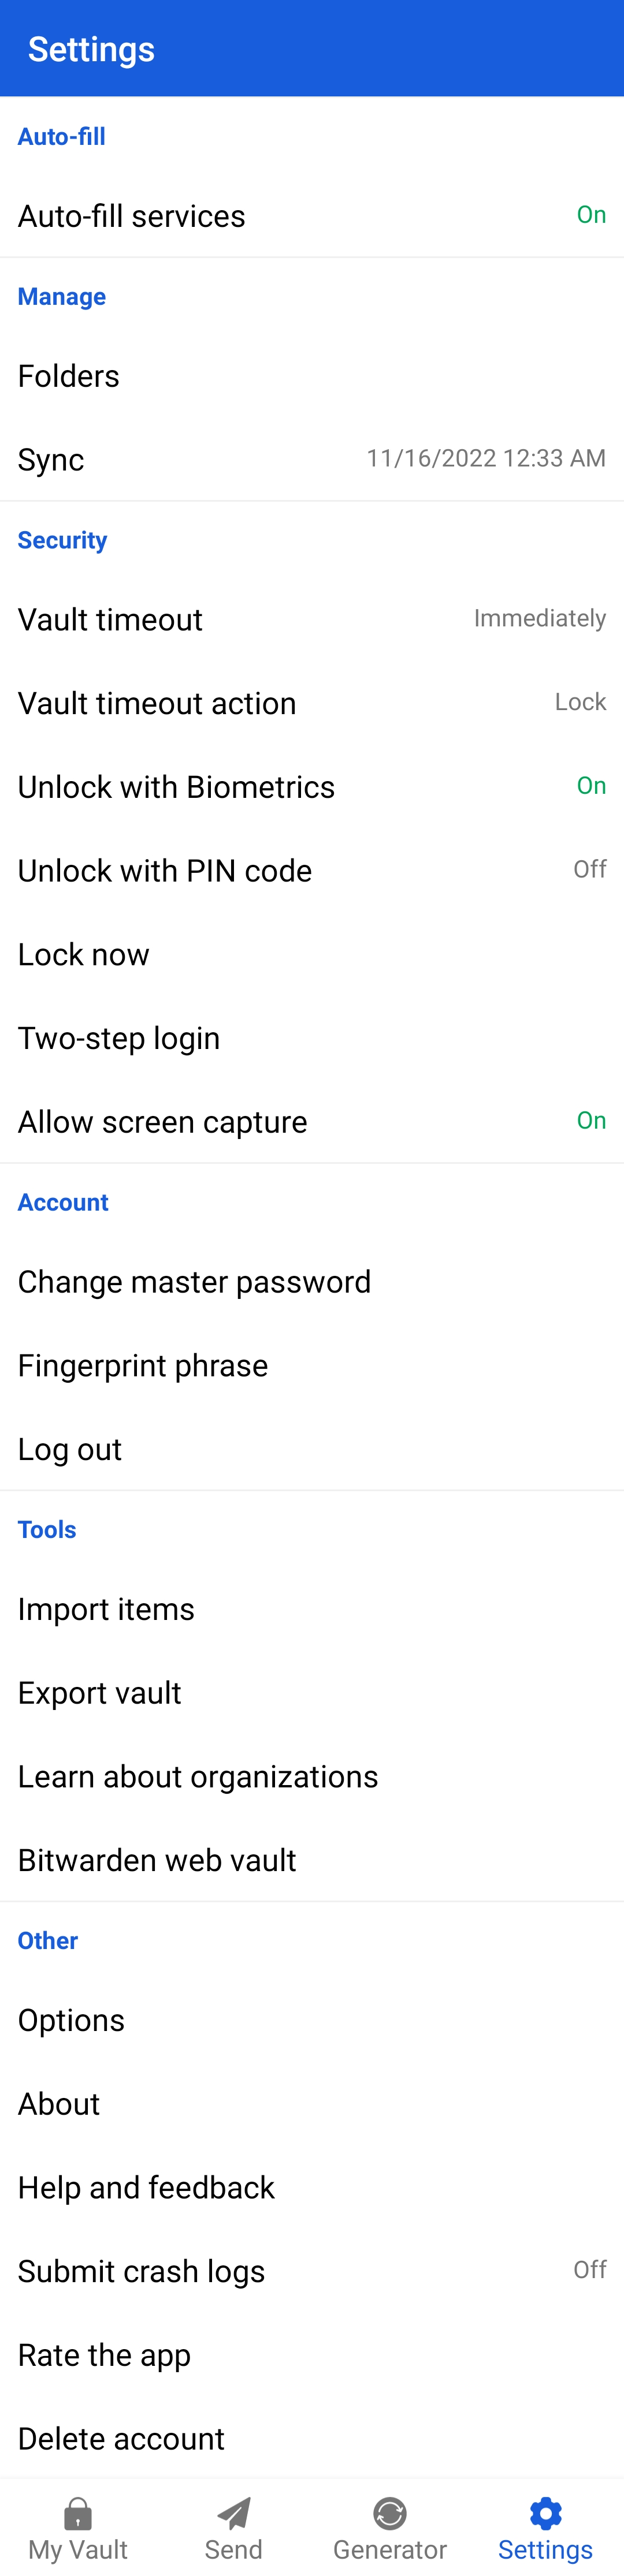
\includegraphics[height={0.935\textheight}]{gfx/bitapp/bitapp-settings-longer.png}}
        \caption{Pantalla de configuración. \href{https://play.google.com/store/apps/details?id=com.x8bit.bitwarden}{De la app de Bitwarden.}}
        \label{fig:bitapp-config}
    \end{figure}
    \columnbreak

     La funcionalidad que aporta InputStick es también un método de inicio de sesión, por lo que podríamos usar la misma estructura para este proyecto y poner la configuración en la pantalla de ajustes, debajo del servicio de auto rellenado.

    También podemos encontrar en la pantalla de Opciones (Figura \ref{fig:bitapp-options}), a la que se accede desde los ajustes, que los servicios de auto rellenado tienen también aquí parte de su configuración. Esta configuración define en qué \glspl{uri} mostrar el \textit{pop-up} del servicio de auto rellenar, también define si registrar como un \gls{login} nuevas entradas. Sin embargo la naturaleza de InputStick es distinta y no es totalmente automático, no existe esta comunicación bidireccional, siempre es unidireccional por el comportamiento del protocolo \gls{hid} mencionado anteriormente, el proceso de inicio de sesión seguirá siempre este orden:
    \begin{enumerate}
        \item Acceder al sitio donde se pretende introducir los credenciales.
        \item Poner el enfoque en el campo de texto que se quiera rellenar-
        \item En el móvil abrir la \gls{vault}.
        \item En la \gls{vault} buscar el \gls{login}.
        \item En el \gls{login} pulsar el botón de enviar.
    \end{enumerate}

    Es por ello por lo que no vamos a añadir ningún campo de configuración en esta pantalla, si no que crearemos una pantalla por separado y se accederá directamente desde la pantalla de Ajustes, teniendo así toda la configuración en la misma ubicación.

    Adicionalmente, deberemos también añadir en esa pantalla una forma de activar o desactivar el servicio, lo cual activará o desactivará los botones para enviar a InputStick.

    En resumen, los objetivos que se plantean son:
    \begin{itemize}
        \item Múltiples botones para enviar a InputStick.
        \item pantalla de ajustes con:
        \begin{itemize}
            \item Interruptor para activar o desactivar la funcionalidad.
            \item Selector de disposición.
            \item Selector de velocidad de escritura automática.
        \end{itemize}
    \end{itemize}
    \vfill\null % relleno
    \columnbreak
    \begin{figure}[H]
        \centering
        \frame{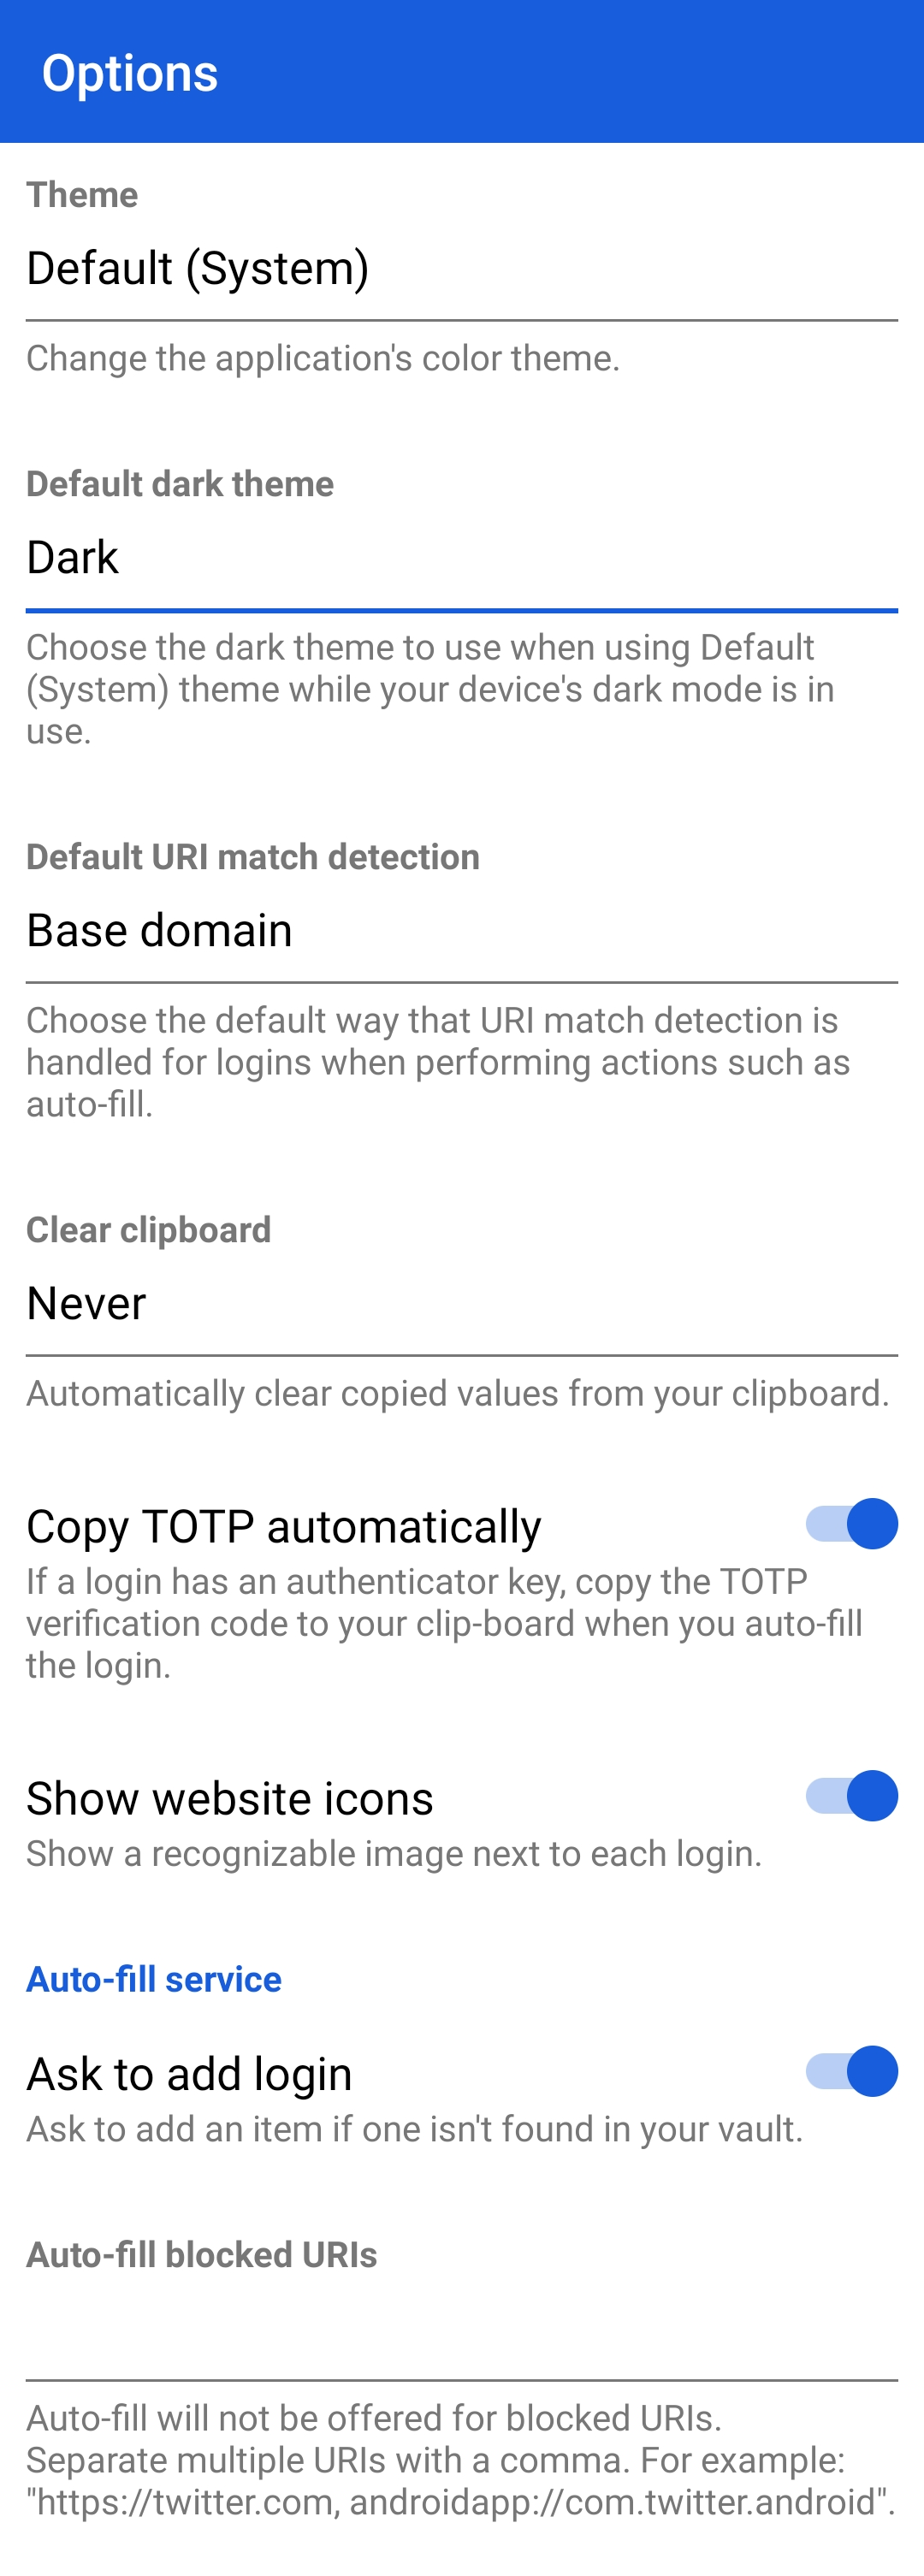
\includegraphics[width={0.785\columnwidth}]{gfx/bitapp/bitapp-options-longer.png}}
        \caption{pantalla de opciones. \href{https://play.google.com/store/apps/details?id=com.x8bit.bitwarden}{De la app de Bitwarden.}}
        \label{fig:bitapp-options}
    \end{figure}
\end{multicols}

\subsubsection{Casos de uso}
Antes de comenzar con el código, es necesario analizar los casos de uso, en la figura \ref{fig:casos} podemos ver un esquema \gls{uml} explicándolos. De forma general casos son enviar campos, elementos del generador y configurar los ajustes.
\begin{figure}[H]
    \centering
    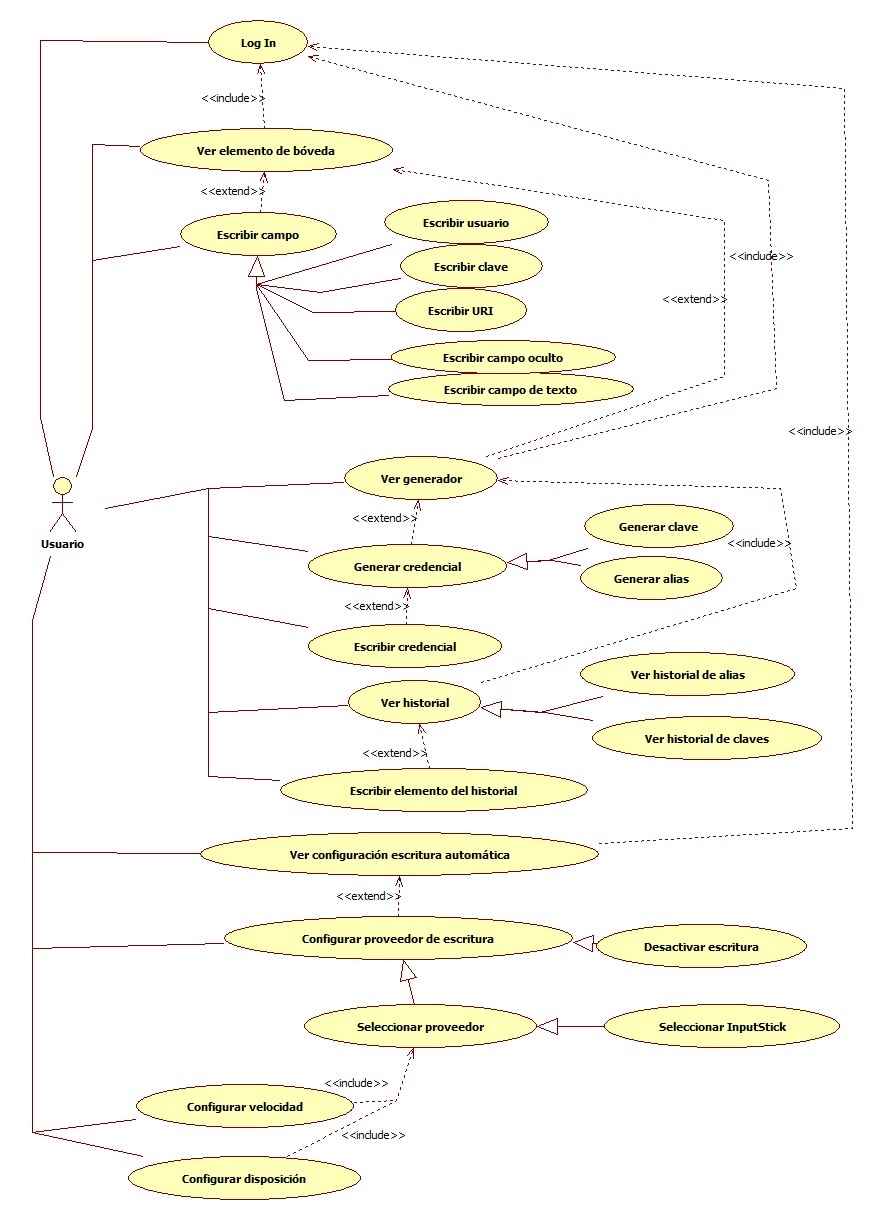
\includegraphics[height={0.935\textheight}]{gfx/casos.jpg}
    \caption{Casos de uso. Realización propia}
    \label{fig:casos}
\end{figure}


\subsubsection{Esquema}
\begin{figure}[H]
    \centering
    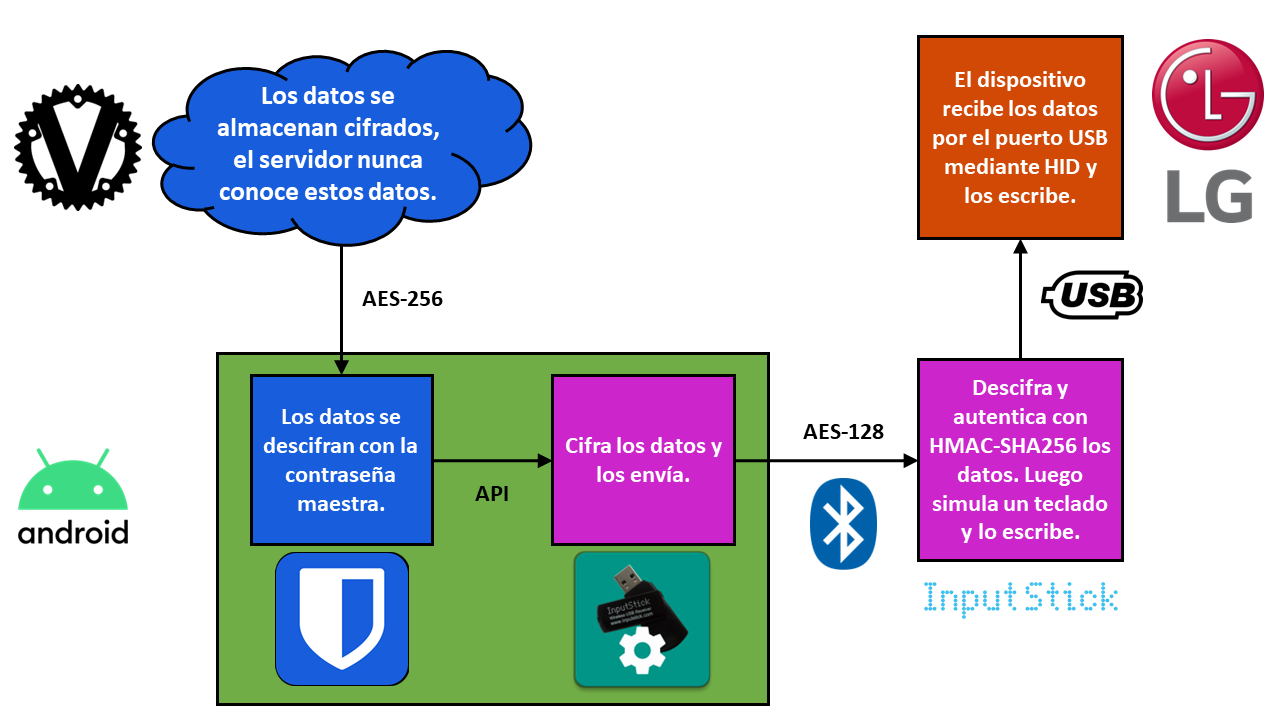
\includegraphics[width=\textwidth]{gfx/Diagrama2.png}
    \caption{Diagrama de conexiones teórico. Realización propia.}
    \label{fig:diagrama}
    El logo de LG representa una \textit{Smart TV}, a modo de ejemplo, pero es sustituible por cualquier dispositivo compatible con \gls{usb} \gls{hid}.
\end{figure}

 La figura \ref{fig:diagrama} ilustra el mapa de conexiones. El servidor de Bitwarden (en nuestro caso Vaultwarden) almacena los datos cifrados, el servidor desconoce por completo la clave para descifrarlos. Estos datos sólo son descifrados en los clientes los cuales le solicitan los datos a Bitwarden. Luego, cuando el usuario decide enviar una clave a InputStick esta se volverá a cifrar para su transmisión por Bluetooth, este proceso lo lleva la app InputStickUtility, a la cual se le transmite la información mediante la \gls{api} InputStickBroadcast\footnote{El nombre pueda dar a entender que los datos se envían a todas las apps, no es así. La llamada a \href{https://github.com/inputstick/InputStickAPI-Android/blob/81d9ce96aa9e4db4f508090f54bea981ffecfcb7/InputStickAPI/src/com/inputstick/api/broadcast/InputStickBroadcast.java\#L208}{type} llama a su vez a \href{https://github.com/inputstick/InputStickAPI-Android/blob/81d9ce96aa9e4db4f508090f54bea981ffecfcb7/InputStickAPI/src/com/inputstick/api/broadcast/InputStickBroadcast.java\#L420}{send}, aquí podemos ver que esto se envía específicamente a la app InputStickUtility.}. Cuando InputStick recibe los datos a escribir los descifra y los envía al dispositivo al que está conectado, usando el protocolo \gls{hid} por \gls{usb}. Finalmente el dispositivo lo escribe en el campo que tenga el enfoque. Se puede observar claramente como los \textbf{nunca} entran o abandonan Android \textbf{sin cifrar}, únicamente cuando se envía la información a InputStickUtility. En la figura \ref{fig:diagrama_real} se muestra como quedaría el resultado final de una forma más práctica y menos esquemática.

\begin{figure}[H]
    \centering
    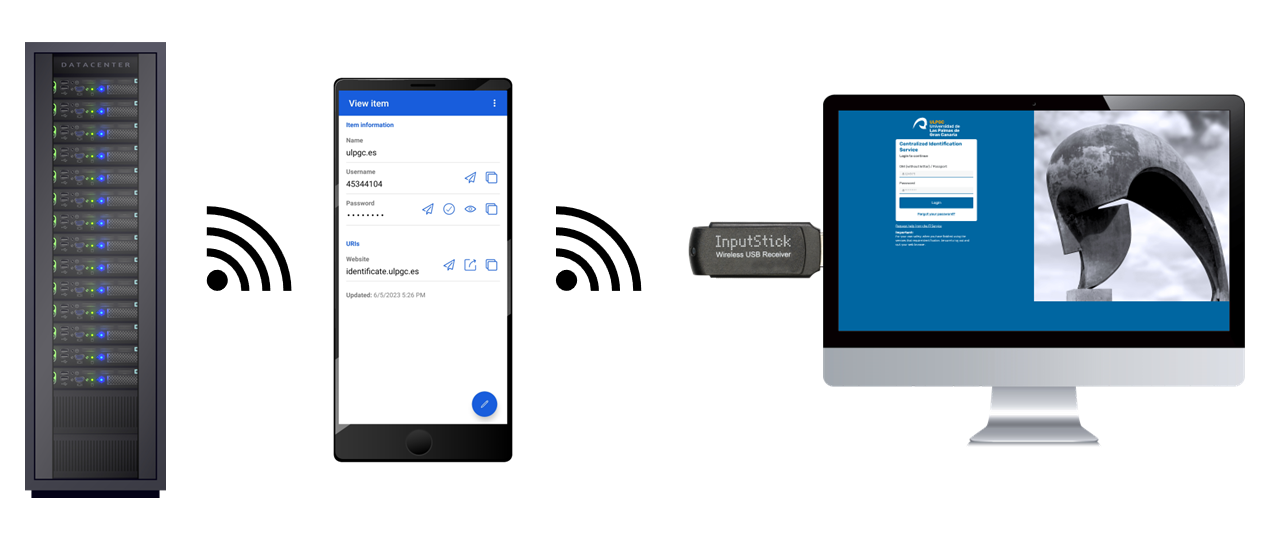
\includegraphics[width=\textwidth]{gfx/diagrama_real.png}
    \caption{Diagrama de conexiones práctico. Realización propia.}
    \label{fig:diagrama_real}
    El ordenador sobremesa es a modo de ejemplo, pero es sustituible por cualquier dispositivo compatible con \gls{usb} \gls{hid}.\newline
    Marco de móvil. Imagen por brgfx en Freepik.com.\newline
    Servidor. Imagen por macrovector en Freepik.com.\newline
    Marco de monitor. Imagen por d3images en Freepik.com.\newline
\end{figure}

% ------------------------
% ------------------------
% ------------------------
% ------------------------

\subsubsection{Model-View-ViewModel}

La app está diseñada con el patrón arquitectónico \gls{mvvm}. Como los patrones \gls{mvc} y \gls{mvp}, este patrón tiene como objetivo abstraer la vista de la lógica.
Este patrón pretende solventar problemas como el grado de acoplamiento que existe en los otros patrones, en \gls{mvc} existe poca independencia entre sus componentes, mientras que en \gls{mvp} ocurre con la vista y el presentador.
Por ello la vista modelo desconoce la existencia de la vista y el modelo desconoce la existencia de la vista modelo.
En este caso, la vista y la vista modelo están enlazadas mediante los campos de datos que son estados que indican a la vista cómo debe presentarse al usuario.
Por otro lado la vista modelo, como intermediaria, mantiene estos campos actualizados recogiendo la información necesaria del modelo, el cual se ocupa de acceder a la base de datos.\cite{García2023mvvm}\cite{Kouraklis2016}

En esta app, el uso de \gls{mvvm} hace que sea bastante fácil y cómodo desarrollarla para distintos Sistemas Operativos como es el caso de Android e iOS, y con la ayuda de Xamarin, esto resulta más claro, ya que ambas versiones comparten el código de la vista, y la vista modelo. Aunque en este proyecto nos centraremos sólo en Android.

\subsubsection{Command}

Para que la vista pueda enviar información a la vista modelo se usa el patrón de diseño command, de esta forma separan el comportamiento de un botón de la vista. Esto se logra convirtiendo solicitudes en objetos, cada objeto es una subclase de la interfaz command\cite{ulpgc.183475}\cite{García2023intro}. Todos los botones tienen una referencia en la vista al comando, el cual se encuentra declarado en la vista modelo. Curiosamente el ejemplo que se usa en libro que se cita está relacionado con el portapapeles (pegar desde el portapapeles), mientras que descubrimos que se usa el patrón command al analizar los botones anteriormente mencionados de copiar al portapapeles.

\subsubsection{Factory method}

Se usa el patrón de diseño factory method para crear diferentes versiones de campos personalizados de un \gls{login}, estos pueden ser booleanos, ocultos, de texto o relaciones. Asumimos que el objetivo es centralizar la creación de estos objetos, pues no se aprovecha el principal beneficio de este patrón, que es evitar especificar la subclase que usar, ya que se le pasa por parámetro un enumerado especificando que subclase se quiere\cite{ulpgc.183475}\cite{García2023intro}.

\subsubsection{Servicios}
La aplicación tiene un sistema de registro de servicios para fácil acceso de distintas funcionalidades en el resto de la aplicación. Se trata de un contenedor de servicios, este es una clase estática, por lo que se puede solicitar acceso a estos servicios desde cualquier parte de la aplicación. No hemos podido encontrar que patrón podría ser este, pero sospechamos que está relacionado con evitar la creación y borrado continuo de objetos.

\subsubsection{\acrfull[hyper=false]{sha}}
En concreto \gls{sha}-256, del grupo \gls{sha}-2 es una función criptográfica de hash, que se usa para verificar la integridad de un mensaje o archivo y por tanto asegurar que no ha sido alterado. Es el estándar actual debido a su eficiencia y  baja posibilidad de colisiones, que se refiere a cuando 2 mensajes distintos devuelven el mismo resultado tras aplicar la función.

\subsubsection{\acrfull[hyper=false]{hmac}}
\Gls{hmac} usa como base una función criptográfica de hash, por ejemplo \gls{sha} y lo combina con una clave simétrica. Se usa para verificar la integridad de un mensaje y por tanto asegurar que no ha sido alterado.

\subsubsection{\acrfull[hyper=false]{aes}}
Es un algoritmo simétrico de cifrado en bloque que tras diversas operaciones como sustitución y permutación cifran el mensaje o archivo. Es el estándar actual debido a su eficiencia y resistencia.